
\documentclass{article}

\usepackage{graphicx}
\usepackage{amsmath}

\title{Variational Autoencoders applied to the MNIST dataset}
\author{
	Ander Arrondo Elizburu \\
	Course: Advanced Machine Learning \\
	\textit{University of Deusto} \\
	Faculty of Engineering
}
\date{\today}

\begin{document}
	\maketitle
	\begin{abstract}
		Abstract here
	\end{abstract}
	
	\section{Introduction}
	This article exemplifies the utility of variational autoencoders (VAE) in computer vision. Specifically, the deep learning algorithms is applied to the MNIST dataset: a set of images containing written numbers.
	\subsection{MNIST dataset}
	The MNIST dataset contains images of hand-written digits in a 28x28 grayscale image format. Figure~\ref{fig:example-digit}, for instance, shows an example of digit \textit{6}. Each image is associated to its proper label. In total, the dataset gathers 70K images of digits with ten possible labels (decimal, from $0$ to $9$).
	\begin{figure}[h]
		\centering
		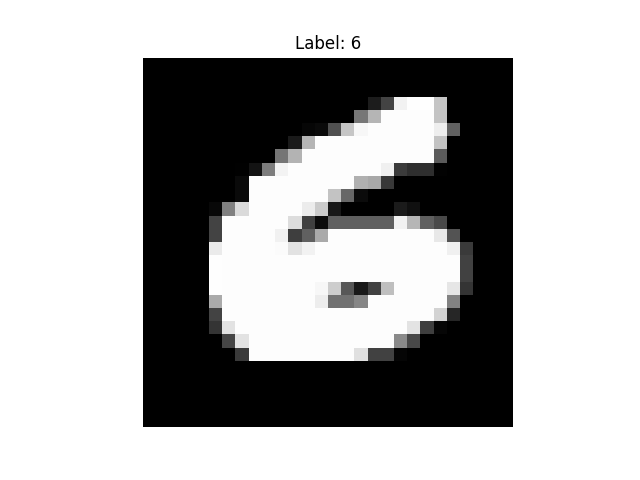
\includegraphics[width=150px]{./plots/single_number.png}
		\caption{An example image of the MNIST dataset.}
		\label{fig:example-digit}
	\end{figure}
	
	The dataset includes various versions of any given digit in order to support generalization. Figure~\ref{fig:multiple-digits} displays a few more examples to illustrate how the datapoints look like. For example, in the figure only one of the images labeled as $1$ has a horizontal line at the bottom.
	\begin{figure}[h]
		\centering
		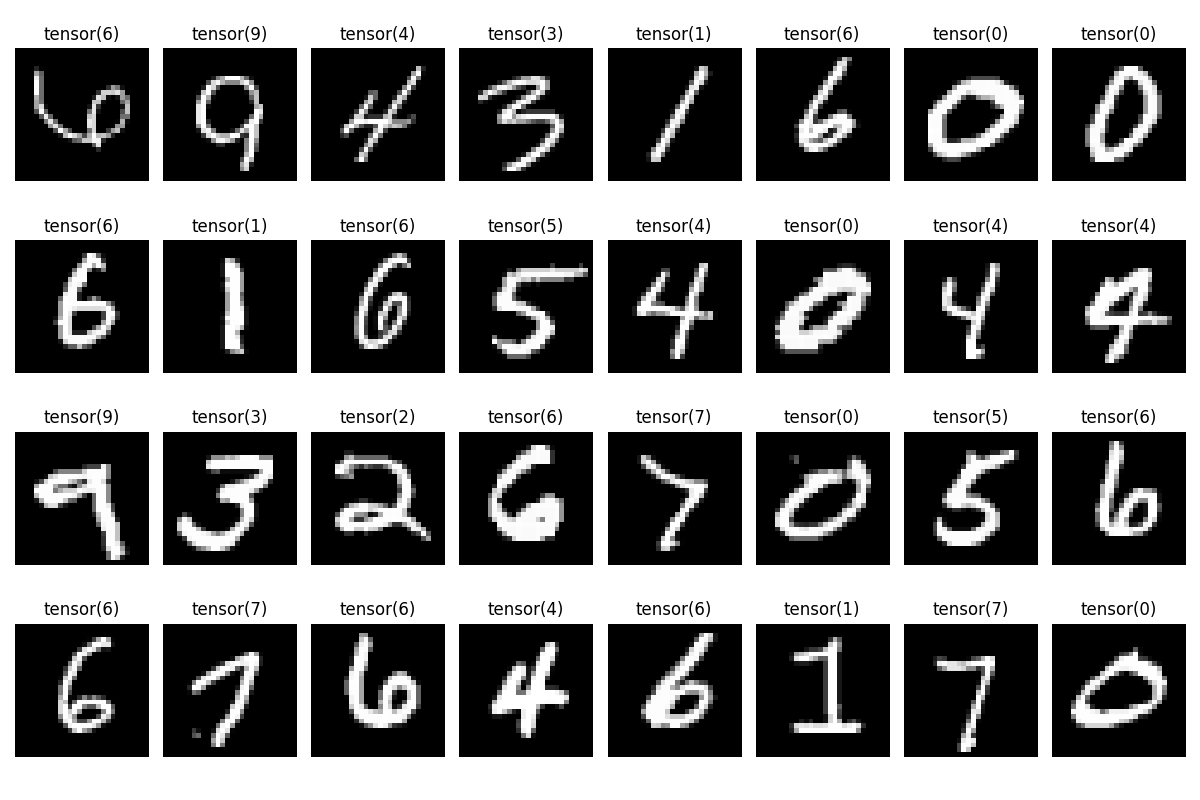
\includegraphics[width=\linewidth]{./plots/multiple_numbers.png}
		\caption{Visual representation of diverse datapoints.}
		\label{fig:multiple-digits}
	\end{figure}
	
	\subsection{Variational Autoencoders (VAE)}
	Variational autoencoders belong to the self-supervised branch inside deep learning. They do not require labels (as supervised learning does), since they learn from the input data itself. In fact, VAEs are a modified version of the autoencoders.
	\subsubsection{Architecture}
	They are divided into three different components: the encoder, the probabilistic latent space, and the decoder. Figure~\ref{fig:vae-diagram} visually represents their structure.
	
	The encoder is, in this case, a multilayer perceptron that takes the original image as input and returns the distribution of the latent space. In general, Gaussian distributions are used to represent the latent space, therefore, the encoder outputs $\mu$ and $\sigma$ for each dimension in it, so that (Equation~\ref{eq:normal-dist}):
	
	The decoder, on the contrary, takes a random latent vector from the probability distribution provided by the encoder and tries to reconstruct the original image based on the information carried by the $z$ vector.
	\begin{equation}
		\mathcal{N}(\mu, \sigma)
		\label{eq:normal-dist}		
	\end{equation}
	\begin{figure}[h]
		\centering
		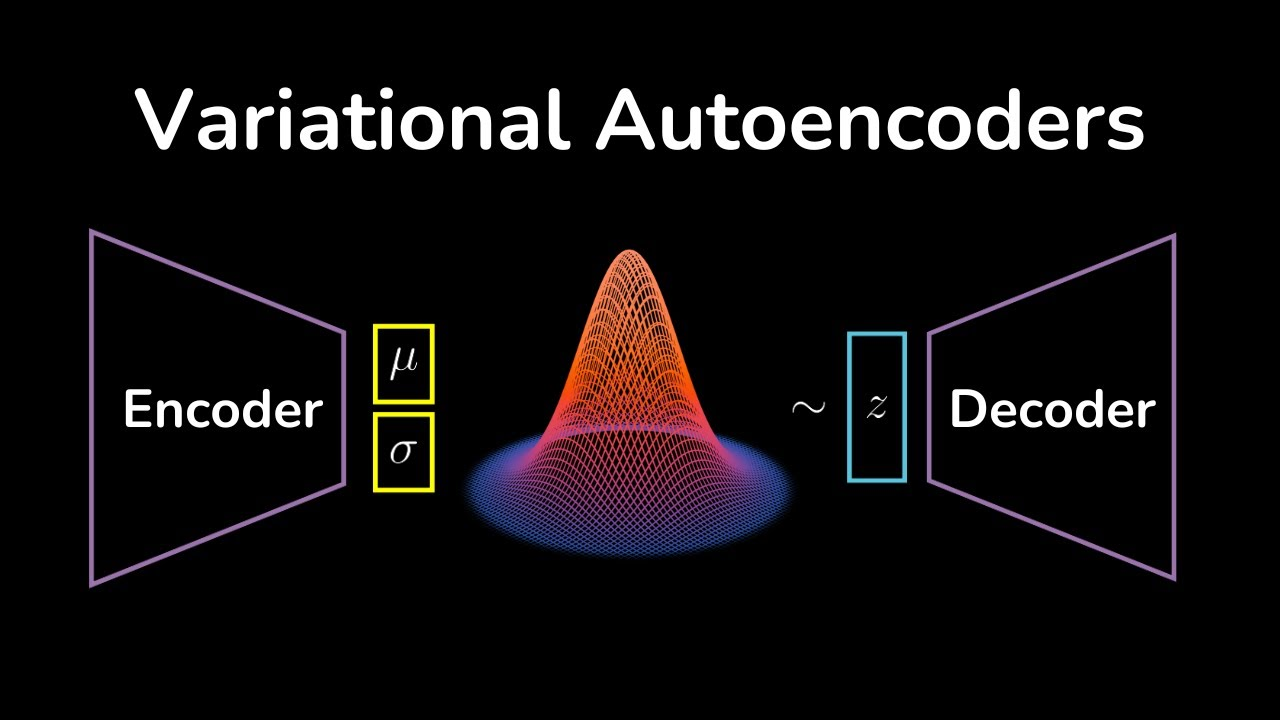
\includegraphics[width=\linewidth]{./plots/vae_diagram.jpg}
		\caption{A visual diagram containing the structure of VAEs.}
		\label{fig:vae-diagram}
	\end{figure}
	\subsubsection{Latent space}
	\subsubsection{Reparameterization and backpropagation}
	
	
	\section{Methodology}
	\subsection{Data preprocessing and splitting}
	\subsection{Hyperparameter optimization}
	
	\section{Results}
	
	\section{Conclusions}
	
	\section{Use of Generative AI}
\end{document}
